% **************************************************
% Document Class Definition
% **************************************************
\documentclass[%
	paper=A4,					% paper size --> A4 is default in Germany
	twoside=true,				% onesite or twoside printing
	openright,					% doublepage cleaning ends up right side
	parskip=full,				% spacing value / method for paragraphs
	chapterprefix=true,			% prefix for chapter marks
	11pt,						% font size
	headings=normal,			% size of headings
	bibliography=totoc,			% include bib in toc
	listof=totoc,				% include listof entries in toc
	titlepage=on,				% own page for each title page
	captions=tableabove,		% display table captions above the float env
	draft=false,				% value for draft version
]{scrreprt}%

% **************************************************
% Debug LaTeX Information
% **************************************************
%\listfiles

% **************************************************
% Information and Commands for Reuse
% **************************************************
\newcommand{\thesisTitle}{A Task-Parallel Sweeping Algorithm for Concurrent Contour Tree Construction}
\newcommand{\thesisName}{Kilian Werner}
\newcommand{\thesisSubject}{Master Thesis}
\newcommand{\thesisDate}{May 24, 2018}
\newcommand{\thesisVersion}{1.0}

\newcommand{\thesisFirstReviewer}{Prof. Christoph Garth}
\newcommand{\thesisFirstReviewerUniversity}{\protect{TU Kaiserslautern}}
\newcommand{\thesisFirstReviewerDepartment}{Department of Computer Science}

\newcommand{\thesisSecondReviewer}{Prof. Heike Leitte}
\newcommand{\thesisSecondReviewerUniversity}{\protect{TU Kaiserslautern}}
\newcommand{\thesisSecondReviewerDepartment}{Department of Computer Science}

\newcommand{\thesisFirstSupervisor}{Prof. Christoph Garth}
\newcommand{\thesisSecondSupervisor}{Prof. Heike Leitte}

\newcommand{\thesisUniversity}{\protect{TU Kaiserslautern}}
\newcommand{\thesisUniversityDepartment}{Department of Computer Science}
\newcommand{\thesisUniversityGroup}{Scientific Visualization Lab}
\newcommand{\thesisUniversityCity}{Kaiserslautern}
\newcommand{\thesisUniversityStreetAddress}{Gottlieb-Daimler-Strasse 36}
\newcommand{\thesisUniversityPostalCode}{67663}

% **************************************************
% Load and Configure Packages
% **************************************************
\usepackage[utf8]{inputenc}		% defines file's character encoding
%\usepackage[english]{babel} % babel system, adjust the language of the content
\usepackage[giveninits=true]{biblatex}
\usepackage[					% clean thesis style
	figuresep=colon,%
	sansserif=false,%
	hangfigurecaption=false,%
	hangsection=true,%
	hangsubsection=true,%
	colorize=full,%
	colortheme=bluemagenta,%
	bibsys=bibtex,%
	bibfile=bib,%
	bibstyle=numeric,%
]{cleanthesis}

\hypersetup{					% setup the hyperref-package options
	pdftitle={\thesisTitle},	% 	- title (PDF meta)
	pdfsubject={\thesisSubject},% 	- subject (PDF meta)
	pdfauthor={\thesisName},	% 	- author (PDF meta)
	plainpages=false,			% 	-
	colorlinks=false,			% 	- colorize links?
	pdfborder={0 0 0},			% 	-
	breaklinks=true,			% 	- allow line break inside links
	bookmarksnumbered=true,		%
	bookmarksopen=true			%
}
\usepackage[T1]{fontenc}
\usepackage{graphicx}
\usepackage{amsmath}
\usepackage{amssymb}
\usepackage{amstext}
\usepackage{amsfonts}
\usepackage{mathrsfs}

\begin{document}  
\pagenumbering{roman}

\pagestyle{empty}				% no header or footers
\begin{titlepage}
	\pdfbookmark[0]{Cover}{Cover}
	\flushright
	\hfill
	\vfill
	{\LARGE\thesisTitle \par}
	\rule[5pt]{\textwidth}{.4pt} \par
	{\Large\thesisName}
	\vfill
	\textit{\large\thesisDate} \\
	Version: \thesisVersion
\end{titlepage}


% ------------------------------------  --> main title page
\begin{titlepage}
	\pdfbookmark[0]{Titlepage}{Titlepage}
	\tgherosfont
	\centering

	{\Large \thesisUniversity} \\[4mm]
	\includegraphics[width=6cm]{gfx/logo} \\[2mm]
	\textsf{\thesisUniversityDepartment} \\
	\textsf{\thesisUniversityInstitute} \\
	\textsf{\thesisUniversityGroup} \\

	\vfill
	{\large \thesisSubject} \\[5mm]
	{\LARGE \color{ctcolortitle}\textbf{\thesisTitle} \\[10mm]}
	{\Large \thesisName} \\

	\vfill
	\begin{minipage}[t]{.27\textwidth}
		\raggedleft
		\textit{1. Reviewer}
	\end{minipage}
	\hspace*{15pt}
	\begin{minipage}[t]{.65\textwidth}
		{\Large \thesisFirstReviewer} \\
	  	{\small \thesisFirstReviewerDepartment} \\[-1mm]
		{\small \thesisFirstReviewerUniversity}
	\end{minipage} \\[5mm]
	\begin{minipage}[t]{.27\textwidth}
		\raggedleft
		\textit{2. Reviewer}
	\end{minipage}
	\hspace*{15pt}
	\begin{minipage}[t]{.65\textwidth}
		{\Large \thesisSecondReviewer} \\
	  	{\small \thesisSecondReviewerDepartment} \\[-1mm]
		{\small \thesisSecondReviewerUniversity}
	\end{minipage} \\[10mm]
	\begin{minipage}[t]{.27\textwidth}
		\raggedleft
		\textit{Supervisors}
	\end{minipage}
	\hspace*{15pt}
	\begin{minipage}[t]{.65\textwidth}
		\thesisFirstSupervisor\ and \thesisSecondSupervisor
	\end{minipage} \\[10mm]

	\thesisDate \\

\end{titlepage}


% ------------------------------------  --> lower title back for single page layout
\hfill
\vfill
{
	\small
	\textbf{\thesisName} \\
	\textit{\thesisTitle} \\
	\thesisSubject, \thesisDate \\
	Reviewers: \thesisFirstReviewer\ and \thesisSecondReviewer \\
	Supervisors: \thesisFirstSupervisor\ and \thesisSecondSupervisor \\[1.5em]
	\textbf{\thesisUniversity} \\
	\textit{\thesisUniversityGroup} \\
	\thesisUniversityInstitute \\
	\thesisUniversityDepartment \\
	\thesisUniversityStreetAddress \\
	\thesisUniversityPostalCode\ and \thesisUniversityCity
}		% INCLUDE: all titlepages
\cleardoublepage

\pagestyle{plain}				% display just page numbers
\begin{abstract}
Topological abstractions like the contour tree play an important role in visualization and analysis of large datasets. They are also computationally expensive and techniques for parallelising and/or distributing of construction methods become more and more crucial when visualizing contemporary, complex datasets with respect to the ever growing available hardware capabilities. However most distributed approaches rely on the sequential, original algorithm for computation, limiting their scalability and load balancing capabilities. More recent decentralized approaches show better performance both in sequential and parallel settings. These approaches however rely on partial ordering or shared memory limiting scalability and feasibility in distributed hardware environments. We will examine the consequences of breaking up this local ordering, constructing a novel, task-parallel algorithm without the need to order. Further this algorithm will be compared to both classic and ordered task-parallel solutions to test feasibility of this approach. Utilizing the newly won independence from ordering, an adaption of the new principle to SIMT architecture is developed for demonstration purposes.
\end{abstract}		% INCLUDE: the abstracts (english and german)
\cleardoublepage
\cleardoublepage
%
\setcounter{tocdepth}{2}		% define depth of toc
\tableofcontents				% display table of contents
\cleardoublepage

\pagenumbering{arabic}			% arabic page numbering
\setcounter{page}{1}			% set page counter
\pagestyle{maincontentstyle} 	% fancy header and footer

\chapter{Introduction}
Contemporary scientific datasets and simulations have become comparably large and complex and continue to grow in size and complexity, utilizing the ever developing hardware capabilities of large clusters. As datasets grow, so does the need for data analysis algorithms, allowing for automatic simplification and visualization of data. Topological algorithms play a major role in this process, as they allow to identify relevant features without human interaction, which would be not feasible for concurrent, raw datasets. For example the information represented in an augmented contour tree of a scalar field allows for automatic simplification while maintaining relevant features. 

However, traditional contour tree computation algorithms are inherently sequential and all contemporary contour tree construction algorithms targeted towards distributed hardware settings utilize strictly data-parallel approaches, dividing the data and running traditional, sequential calculations on each subdivision. These approaches share a limitation on scalability and a lack of load balancing capabilities. 

In the last two years multiple approaches from a more decentralized, inherently parallel perspective were undertaken, resulting in more performant and scalable solutions for different architectures. Most of these recent approaches share a common core perspective \cite{base}, that allows for decentralized identification of merge tree nodes.

However none of those recent works targeted truly distributed settings, as they either relied on partially ordering, shared memory or SMP hardware environments.

The common theoretical basis for the recently developed, decentralized approaches is recaptured and extended upon in this Thesis. This core idea can be formulated as understanding a set of necessary and finally sufficient conditions for a vertex to represent a saddle in a merge tree. This set of conditions was used by recent solutions in varying degrees to enable a decentralized, non-global viewpoint leading towards more inherently parallel solutions, instead of traditional data-parallel divide and conquer strategies. 

One of these solutions \cite{FTM} was even able to formulate augmented merge tree construction as a task-parallel problem, however remained unfit for distributed settings because of the dependency on locally ordered progression within each task. 

To clear the way towards a task-parallel, distributed, augmented contour tree construction algorithm, the consequences of avoiding partial orderings and dependencies on shared memory in merge tree construction are evaluated, leading to a novel merge tree construction algorithm with feasibly distributable properties. As this novel approach does discard certain assumptions present in related work, some additional algorithmic complications are introduced. To minimize the performance impact of these complications possible design strategies and implementation techniques are evaluated. 

Finally, to demonstrate the capability of the novel approach to perform well in hardware settings, that are not feasibly utilized with data-parallel or locally ordered approaches, a hardware-accelerated variant of the solution is developed and benchmarked on an NVIDIA GPU. 

\chapter{Establishing a Theoretical Basis} \label{sec:num2}
Constructing a contour tree by constructing join and split tree first and then building the contour tree from them was introduced in \cite{orig} and has since then become a well established basis for almost all algorithms concerned with contour tree construction. The final merging step of the two merge trees has seen little to no improvement since its introduction, as it is both inherently sequential and computationally inexpensive with respect to the overall contour tree construction times. In this thesis we will therefore concentrate on merge tree construction only, a parallel merge step is for example well described in \cite{Carr}.

The trend to approach merge tree construction from a decentralized point of view \cite{base}, focusing on critical points and monotone paths connecting them, can be observed in most of the recent work in this field \cite{Carr}, \cite{FTM}, \cite{adhoc}, \cite{Maadasamy}. In this section we will be looking into the definitions regarding merge tree construction to understand this decentralized approach and the set of necessary and finally sufficient conditions at its core. With this perspective in mind the approach in \cite{FTM} comes as a natural parallelization of the original ordered union-find algorithm in \cite{pascucci1}. This then leads us to the question of why local ordering is present in \cite{FTM} and how the concept could be adapted to no longer depend on it. The answers to this question will then lead to the foundation of our novel merge tree construction algorithm.

\section{Merge Tree Definition}
Consider a smooth, real-valued function \(f\) on a manifold \(M\). A merge tree is either a join or a split tree, the following definition covers the join tree, the definition of a split tree follows similarly with super-level sets instead of sub-level sets. 

A join tree represents the development of the sub-level set \(M^{a} = f^{-1}(-\infty, a]\) with growing \(a\), with respect to the number of connected components. There are two types of events that can change the number of connected components in the developing sub-level set at a value \(a\): Creation of a new component and the merging of two such components. These events are represented by the two types of nodes in a join tree: leafs representing minima (extrema in general) and inner nodes representing join nodes (saddles in general). 

Let in the following \(M'^{a} = f^{-1}(-\infty, a[\) be the sub-level set just "before" a. While in general \(f^{-1}(a)\) may contain more than one point, when defining the two event types we will refer to a point \(p^a\) corresponding to \(f^{-1}(a)\). This is meaningful because, if \(f^{-1}(a)\) contains more than one point, at most one of those points will fit either of the following criteria, because \(f\) is assumed to be a Morse function.
\paragraph{Minima/Extrema} If \(p^a\) has at least one neighborhood in \(M\) without any points whose image under \(f\) are part of the sub-level set \(M'^a\), then \(p^a\) corresponds to a new connected component of \(M^a\). In a join tree every value \(a\) with this property will be represented by a leaf and called minimum.  
\paragraph{Join Nodes/Saddles} If all neighborhoods in \(M\) of \(p^a\) include points whose images under \(f\) are part of at least two different connected components of \(M'^a\), then \(p^a\) creates a connection between those connected components, joining them into one connected component of \(M^a\). In a join tree every value \(a\) with this property will be represented by an inner node, sharing an edge with the minima or inner nodes representing the newly joined components. These nodes are called join nodes and the edges are called arcs.

\paragraph{}For the sake of illustration one can let \(M\) be the $\mathrm{R}^2$ and visualize the values of \(f\) as height of a smooth landscape embedded in $\mathrm{R}^3$. Cutting through this landscape with a plane with height \(a\) and discarding any portions "above" the cut leaves us with the sub-level set of \(a\). With growing \(a\) this cutting plane rises and uncovers a growing portion of the landscape. When just considering the number of connected components of this uncovered part, the two events become apparent: At some point the plane will cut a "valley" for the first time, creating a new component and at some other point two rising valleys may come in contact for the first time at what would look like a hill ridge or saddle.

\section{Augmented Merge Tree and Scope}
The definition above is far more general, than needed in practical applications. The scope of this thesis and the introduced algorithms will cover discretized data sets with a finite number of vertices and a known neighborhood relation between them, approximating the abstract manifold above. 

\paragraph{Augmented Merge Tree} This limitation to a finite point number allows for the definition of the augmented merge tree: A merge tree is augmented, if -in addition to minima, join nodes and their connections in the tree- for every point in the data it is known, which connected component of their sub-level set they lie within. This can be represented by relating each point in the data to one edge in the merge tree. 

\begin{figure}[h!]
\centering
\includegraphics[width=0.7\textwidth]{figures/Ambiguity.pdf}
\caption{Illustration of the possible existence of in-cell saddles on interpolated datasets and comparison to the abstraction chosen in this Thesis.}
\label{fig:csc}
\end{figure}

\paragraph{} Further, in this thesis we will disregard information about cells and instead work with the abstraction of a simplical 1-complex (or a graph). It is possible for saddles to exist inside of cells when working with a volumetric abstraction, as for example in the case of trilinearly interpolated cubics. However in the context of augmented merge trees this scenario is not meaningful. Arcs between those saddles would be empty regarding the augmentation and those saddles could not be identified with a vertex of the input data. Additionally most data sets are prone to noise, thus it is common to simplify the resulting merge trees. Sub-resolution arcs are prone to aliasing and should not be present after simplification. 

Lastly real-world data usually does not comply to the requirement of \(f\) being a Morse function. Luckily on a piecewise linear simplical 1-complex with finite vertices and edges, any real-valued function on the vertices can be made Morse by perturbating duplicate function values, making \(f\) injective. This process is called simulation of simplicity and is usually done by resolving comparisons of equal function values by comparing the index of their vertex.

\section{Decentralized Observations}
When trying to compute a merge tree for this kind of scope the traditional approach in \cite{orig} was to mimic the growth of \(a\) by sequentially visiting every vertex in ascending order of their function value and keeping track of the connected components of the growing datastructure \cite{pascucci1}. However in recent work this global, sequential point of view was replaced by a more decentralized approach, that focused on the question: Can we identify extrema, saddles and arcs independently of the global state? 

\subsection{Identifying Extrema}
Identifying extrema as in the sense of merge trees is actually possible by observing only the local neighborhood of a vertex. If a vertex \(v\) has a function value \(a\) smaller than all function values of its neighbors it is a minimum and will appear as a leaf in the join tree. In other words, if all vertices connected to \(v\) cannot be part of the sub-level set of \(a\) because of their larger function value, then all sub-level set components of \(a\) can only contain vertices not connected to \(v\). Thus \(v\) will create its own sub-level set component and correspond to a minimum as in the definition above.

\subsection{Identifying Saddles}
Identifying a saddle vertex is a much more complicated task and is not possible via his direct neighbors only. 

However a necessary condition can be observed: 

\paragraph{First Condition} Since a saddle \(v\) connects two previously unconnected components of the sub-level set of its value \(a\) it must be directly connected to vertices belonging to these connected components. Thus it needs at least two neighboring vertices with function values smaller \(a\) that are not direct neighbors of each other. Lets call such \(v\) a saddle candidate. See Figure \ref{fig:sc}.

\begin{figure}[h!]
\centering
\includegraphics[width=0.7\textwidth]{figures/SaddleCandidatesCrop.pdf}
\caption{Saddle candidates in a 2D exemplary dataset and their respective smaller neighbors, that are not directly connected to each other.}
\label{fig:sc}
\end{figure}

\paragraph{}
Actually this necessary condition is closely related to a sufficient condition. If these at least two neighboring vertices with function values smaller \(a\) are not only not direct neighbors, but can also not reach each other in the restriction of the data to the sub-level set just before \(a\), then they are not part of the same connected component before meeting at \(v\) thus \(v\) is a saddle, joining the two components. This allows for the identification of saddles by starting a breadth first search through the mesh at all neighbors of \(v\) with a smaller value than \(a\) stopping at any vertex with a higher value than \(a\). If some of these breadth first searches terminate with disjoint sets of visited vertices, \(v\) is a saddle. A very similar principle is for example utilized in \cite{Maadasamy}.

\subsection{Identifying Arcs}
However saddles can also be identified alongside the arcs connected to them. For this, the sufficient condition above will be reproduced by two additional necessary conditions, that can be checked more easily. Consider the following observation: 

\paragraph{Lemma 1} Vertices that are not reachable by a monotone path from a minimum, cannot belong to the same sub-level set component as the minimum, in sub-level sets for lower values than that of the saddle of that minimum. They cannot belong to the "initial" component of the minimum.

\paragraph{Proof Concept} 
If there exists no such monotone path from a minimum \(m\) to a vertex \(v\), then on every path from \(m\) to \(v\) there is at least one in-between vertex with a larger value than \(v\) (and also than \(m\) because \(m\) is a minimum and thus smaller valued than any of its neighbors). Let \(a\) be the smallest of the values of these larger valued in-between vertices. Then \(m\) and \(v\) cannot be part of the same component of the sub-level set just before \(a\), because all connecting paths between them are still interrupted by the in-between vertices that are not yet part of the sub-level set. Since \(p^{a}\) is now a possible saddle at which the components of \(m\) and \(v\) merge with each other, their actual saddles are either both \(p^a\) or will have a lower value than \(a\). In both cases at the level of their respective saddles the sub-level set components of \(m\) and \(v\) can not have joined yet.

\paragraph{Lemma 1.1} A Vertex \(v\) that is reachable by a monotone path from a minimum \(m\), will be part of the same sub-level set component as \(m\) for every possible sub-level set.

\paragraph{Proof Concept}
Assume there is a value \(a\) with the sub-level set \(M^a\), such that \(v\) and \(m\) belong to different connected components in \(M^a\). Then there is no path between \(v\) and \(m\) in \(M^a\). Therefore on every path between \(v\) and \(m\) in \(M\) there has to exist at least one vertex with a higher value than \(a\). This either means, that no monotone path between \(v\) and \(m\) exists in \(M\) or \(v\) has a higher value than \(a\) too. In the second case \(v\) would not be part of any connected component in \(M^a\), thus Lemma1.1 holds.

\paragraph{}
This leads us to a very important, second necessary condition for a vertex \(v\) to be a saddle for a minimum \(m\):

\paragraph{Second Condition} In order for \(v\) to be the saddle for \(m\), at least one of the smaller neighbors of \(v\) must be not reachable through monotone paths from \(m\). Lets call saddle candidates, that fulfill this second condition for at least one minimum "connecting" saddle candidates.

If \(v\) was not connecting, none of the smaller neighbors of \(v\) could belong to a different sub-level set component just before \(v\) than \(m\) so \(v\) could not connect any previously unconnected components with the component of \(m\).

\begin{figure}[h!]
\centering
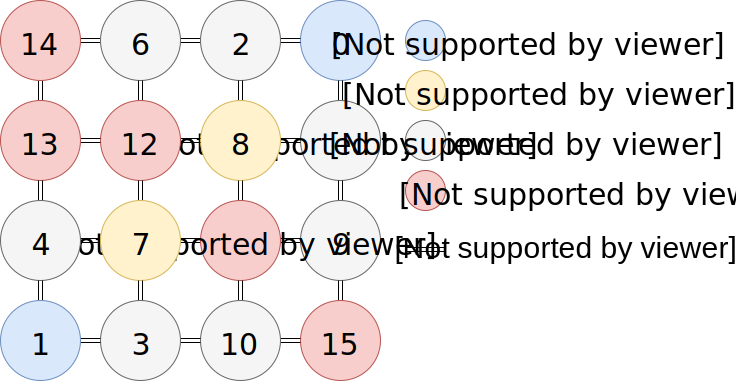
\includegraphics[width=0.7\textwidth]{figures/ConnectedSaddleCandidates.pdf}
\caption{Connecting and non-connecting saddle candidates in a 2D exemplary dataset. Note that 14 is connecting w.r.t. 1 but not w.r.t. 0. and 13 is connecting w.r.t. 0 but not w.r.t. 1}
\label{fig:csc}
\end{figure}

\paragraph{Third (final) Condition} Among all connecting saddle candidates for \(m\) the one with the smallest value is the saddle for \(m\).

\paragraph{Proof Concept}
Consider a connecting saddle candidate \(s\) for \(m\). \(s\) has at least one smaller neighbor \(v\), that is initially not part of the same connected component as \(m\). The only possibility for \(v\) and \(m\) to be part of the same sub-level set component in the sub-level set just before \(s\), is for the initial sub-level set components of \(v\) and \(m\) having already joined at another saddle, with a smaller value than \(s\). If \(s\) is the vertex with the lowest value among all vertices fulfilling necessary conditions to be a saddle for \(m\), then this possibility vanishes and \(s\) will join the components of \(v\) and \(m\).

\paragraph{}
Having finally found a sufficient condition for a vertex \(v\) to be the saddle for a minimum \(m\), one last question remains. How do we find the smallest connecting saddle candidate for a given minimum \(m\)? This is where most of the recent work, based on the above set of conditions take different approaches. Most of them rely on monotone paths, which is due to an additional, necessary condition for saddles:

\paragraph{Lemma 2} There has to exist a monotone path from every minimum \(m\) to its saddle \(s\). 

\paragraph{Proof Concept}
If there exists no such monotone path, then on every path from \(m\) to \(s\) there would be at least one vertex \(v\) with a smaller value than at least one of the vertices on any path from \(m\) to \(v\). Due to Lemma1 \(v\) has to be in a different connected component than \(m\) before reaching \(s\). Since there exist such a \(v\) on every path from \(m\) to \(s\), the component of \(m\) would have to join with at least one of their components before reaching \(s\), thus leading to a contradiction, since \(s\) can no longer be the saddle that merges the component of \(m\).  

\paragraph{}
The three conditions and Lemma 2 lead to the following conclusion: The saddle for a minimum \(m\) is the vertex with the smallest value, that is reachable through monotone paths from \(m\) and at least one other minimum. 

This conclusion can also be extended to saddles of other saddles, since contracting all vertices that belong to the sub-level set component of a join node to one point, this point can be treated as a minimum.

\section{Global Ordering and Local Ordering}
From that new perspective the classic, global algorithm \cite{orig} still makes sense: 

Visiting all vertices in ascending order of their value will in fact follow ascending paths, starting in minima. This approach will always continue the monotone path with the smallest valued, next-to-visit vertex between all minima. In this case, keeping track of what minimum is able to reach which vertex through monotone paths coincides with keeping track of the sub-level set component growth. This assures, that when reaching a saddle candidate, all possible ascending paths to its smaller neighbors have already been followed. Checking the second condition for the candidate is therefore easily done. Due to the ordered nature of the progression, the first saddle candidate to fulfill the second condition will also be the smallest to do so thus it fulfills the third condition. Thus any visited vertex with at least two smaller neighbors that don't belong to the same component yet is the saddle for these components.

\paragraph{}
However with this new perspective a parallel variant of the algorithm comes as a natural extension: 

Instead of always visiting the smallest valued extension of any component, we are allowed to visit the smallest valued extension of each component in parallel. Extending, per minimum \(m\), the monotone path with the smallest valued next-to-visit vertex will eventually lead to a vertex \(v\) that has a smaller valued neighbor that has not been visited by this minimum monotone paths yet. Since all monotone paths leading to smaller valued vertices than \(v\) has been visited, this smaller neighbor has to belong to a different sub-level set component thus \(v\) is a connecting saddle candidate. Since we always visited the smallest monotonely reachable vertex, \(v\) is also the smallest connecting saddle candidate and therefore the saddle for \(m\). Note, that in this parallel variant of the merge tree construction, at the time a saddle and arc is identified, it is not necessarily known yet which other arcs lead up to the saddle. In other words we identify a join node from each minimum individually, the information which components join together in the node is only available once all minima have identified the join node. The above method is employed by \cite{FTM}.

\section{The Limitations of Ordering}
While the above parallel solution is very performant in practice, the inherent parallelism it exposes is limited by two aspects. 

First, in order to find the edges between inner nodes of the tree, join nodes are treated like minima. This is only possible after contracting the connected component represented by the join node to one vertex. This again is only possible after the represented connected component is identified, thus after all minima that join in the node have identified it as their saddle. This creates a sequential dependency, binding the runtime to scale with the depth of the output, even for optimal parallelism. This sequential dependency however seems inherent for the problem of merge tree construction, since having a notion for connected components existing in the sub-level set before a critical vertex seems to be inevitable. 

Second, starting at each minimum, the smallest monotonely ascending path is followed, thus only one parallel line of execution exists per minimum. The number of parallel lines of execution also decreases over time, as for every at least two minima who identify their join node only one new (contracted) "minimum" starts its search. This leads to a worst case scenario, where the whole dataset contains only two minima starting connected components spanning half of the dataset each. The theoretical parallel speedup that can be reached in this scenario would be limited to two.

This second limitation is also very problematic when trying to implement the solution with the use of hardware acceleration or for distributed settings. This is especially true when splitting the data among the nodes in a distributed setting. Here the restriction of monotone path extensions having to be in order could lead to extreme load imbalance, when most paths lead into the domain of one node. Additionally if a connected component lies on the border between data domains of different nodes the ordered traversal of the monotone paths might force the two nodes to alternately wait for each other to continue at the next smallest vertex.

\section{The Need for Ordering?}
In order to overcome these limitations, it seems desirable to find a solution that does not depend on any order when traversing the monotone paths from the minimum. Lets consider again the role the local ordering plays in finding the saddle. Starting at a minimum \(m\) and following monotonely ascending paths we are searching for the saddle \(s\) of \(m\). \(s\) is the only vertex fulfilling all three conditions.

When reaching a saddle candidate \(s_c\) while following the monotone paths from \(m\) we rely on the progression to be ordered by value to ensure \(s_c\) matches conditions two and three. If among the smaller neighbors of \(s_c\) there is at least one that has not yet been reached by monotone paths from \(m\), we know it will never be reached later on. This is only thanks to the ordered progression. We need this knowledge to employ Lemma1 to \(s_c\) and ensure condition two. When finding a saddle candidate that fulfills condition two, we instantly know it is the smallest among those and fulfills condition three, which is again only thanks to the ordered progression of the monotone paths.

\paragraph{}
So in order to reach the goal of not relying on an ordering of the local searches, but instead being able to follow all monotone paths from \(m\) in parallel, we need another way to evaluate conditions two and three. A naive solution would be to follow all monotone paths from \(m\) and keeping track of any saddle candidates. Once the search completely terminates (having run into local maxima) we can check the saddle candidates for condition two, because every vertex not visited by this complete search is not reachable from \(m\) via monotone paths. From all saddle candidates fulfilling condition two the minimum can be selected and the saddle is found. This naive approach exposes a far greater inherent parallelism and will theoretically outperform the ordered approach in a perfectly parallelised environment. However while the ordered approach guarantees that every vertex is only visited once, this naively unordered solution would result in large portions of double work. The question arises: Is there a natural boundary for the unordered search that guarantees no double work is done?

\section{Ascending Manifold Boundary} \label{ssec:num1}
Consider the set \(A_m\) of all vertices from where all monotonely descending paths end in a minimum \(m\). The other way around no vertex in \(A_m\) can be reached through monotonely ascending paths from any minimum other than \(m\). \(A_m\) is a connected subgraph in the input data. 

\paragraph{Lemma 3} Every neighbor \(v\) of any vertex \(k\) in \(A_m\) is a saddle candidate.

\paragraph{Concept of Proof}
\(v\) is not part of any set \(A_n\) for an arbitrary \(n\). Otherwise the larger of \(v\) and \(k\) could be visited by either \(m\) or \(n\) respectively, which contradicts their existence in \(A_n\) or \(A_m\) respectively. Thus \(v\) can be reached from at least two different minima through monotonely ascending paths. Also \(k\) has to have a smaller value than \(v\) otherwise \(k\) could be monotonely reached by at least the same set of minima that can reach \(v\). Since \(v\) can be monotonely reached from more than just \(m\) and \(k\) as one of its smaller neighbors is only reachable from \(m\), \(v\) needs to have at least one additional smaller neighbor \(l\) that can be monotonely reached by at least one minima other than \(m\). \(k\) and \(l\) cannot be direct neighbors for the same reason \(v\) and \(k\) could not be.

\paragraph{Lemma 4} The smallest vertex \(v\) among the neighbors of vertices in \(A_m\) fulfills the second and third condition.

\paragraph{Concept of Proof}
Due to the concept of prove above \(v\) must have a neighbor \(l\) with a smaller value than \(v\), that is reachable by at least one minimum other than \(m\). Since \(l\) is smaller than \(v\), \(l\) cannot be reached by a monotone path from \(m\) through \(v\). Due to Lemma3 every monotone path from any vertex inside \(A_m\), including \(m\), to any vertex outside of \(A_m\) must contain a saddle candidate, all of which are larger than \(v\) and thus \(l\). Therefore no path from \(m\) to \(l\) can be monotone and thus \(v\) fulfills the second condition. Additionally \(v\) also fulfills condition three, as there can be no monotonely reachable vertices outside of \(A_m\) smaller than \(v\) (and saddles need to be monotonely reachable due to Lemma2).

\paragraph{}
In other words all monotonely ascending paths starting in \(m\) will run into saddle candidates at one point and the smallest of these is the saddle for \(m\). Thus an unordered growth of any and all monotonely ascending paths starting in \(m\) can be terminated at the surrounding saddle candidates and checking for the second condition can be skipped. Does this solution guarantee that no double work is performed while traversing the monotone paths?
  
\begin{figure}[h!]
\centering
\includegraphics[width=0.7\textwidth]{figures/AscendingManifold.pdf}
\caption{Ascending Manifolds of two local minima in an exemplary 2D dataset. Manifold boundaries are not identical, but do overlap.}
\label{fig:am}
\end{figure}
  
The sets \(A_m\) correspond to the Morse theory concept of the ascending manifold of \(m\). Once a join node \(s\) and its sub-level set component are contracted to a minimum, the set \(A_s\) correspond to the ascending manifold of \(s\). Thus every vertex is visited once for each ascending manifold it belongs to. Since ascending manifolds do not overlap and form a partition of the domain, it is guaranteed that no double work is performed while visiting the vertices.

\paragraph{}
These final thoughts extend upon the necessary conditions above and portray saddles as the smallest vertices on the ascending manifold boundary of a minimum. This perspective is latently utilized in \cite{Carr} and builds the basis for the novel algorithm presented in this Thesis.

\chapter{Related Work}
In the following a general overview of the efforts towards parallel contour tree construction are presented in semi-chronological order to understand how data-parallel approaches emerged and finally gave way to the recently developing trend of decentralized and task-parallel approaches. Now that the common theoretical basis for most of this recent work is recaptured, the actual application of it in each of them can be explained.

\paragraph{Sequential Basis} 
The basis for most if not all following work is the original algorithm for constructing augmented contour trees in all dimensions \cite{orig}. The general layout of this algorithm is to perform two completely ordered sweeps over the dataset, one ascending and one descending. This constructs a join or split tree respectively, by keeping track of the development of level-sets using a union find datastructure. Later on the two resulting merge trees are combined to create the contour tree. This last step is performed in a sequential manner, requiring global information of the merge trees. Since this is rarely the bottleneck for computation times, to this day few efforts were undertaken to parallelize or distribute this step.

\paragraph{The first approach} to a parallel contour tree computation was done by Pascucci et al. \cite{pascucci1}. It is a prime example of traditional data-parallel solutions: First, the mesh is divided into chunks of almost equal size. Second, the split/join tree is computed for each chunk in parallel. Within each chunk the merge tree computation is run sequentially, utilizing the classic, ordered traversal union-find mentioned above. Third, the local join/split trees are composited hierarchically. Each composition is sequential in nature and due to the reduction like communication pattern, there will be idle capacities in the later composition rounds. Finally the gathered join and split tree are merged to form the contour tree in a sequential matter.

\paragraph{Domain space subdivision}
Charles et al. \cite{Charles} take a somewhat different approach. Instead of subdividing the mesh in a spatial manner, they subdivide it using iso level sets. Again within each chunk, a contour tree is computed in the sequential, traditional union-find manner mentioned above. All arcs that lie completely inside the level set of the respective chunk are already correct arcs in the final contour tree. In a similar fashion to \cite{pascucci1} the local trees are now merged hierarchically until the contour tree is complete. 

\paragraph{Distributed Contour Trees}
A recent approach by Morozov et al. \cite{Morozov} is aimed towards a distributed setting and computes a distributed representation of the contour tree, by observing that every vertex lies on exactly one path between a local minimum and local maximum. This approach is in itself quite feasible and would not need adaption to our scenario, but inherently does not produce an actual augmented contour tree for general purpose use cases.

\paragraph{Sweep to Saddle}
The first appearance of the recent decentralized perspective \cite{base} can be found in the field of ad-hoc networks. Sarkar et al. \cite{adhoc} explore the possibility to make an ad-hoc network of sensors aware of the contour tree on the scalar field they measure. In a very similar fashion to \cite{Carr} and the novel algorithm discussed in this thesis, the boundary of the ascending manifold of local minima is extracted and the smallest vertex among this boundary is identified as the saddle in the join tree for that minimum. This is a direct application of the set of necessary conditions for a vertex to be a saddle for an extremum, that form the common theoretical basis for this approach and most of the following. In fact, the solution in \cite{adhoc} can be interpreted as a special case of the novel algorithm presented in this Thesis, when working in an ad-hoc hardware environment.

\paragraph{Maximum lists and path lists}
A different approach is taken by Maadasamy et al. \cite{Maadasamy}. Here the data is iterated over in arbitrary order (and possibly in parallel) finding all critical points and monotone paths from each critical point that is no extremum (so from each saddle) to extrema. This is again based on the necessary conditions that form the common theoretical basis. Saddle-Candidate to extremum relationships are modelled with lists containing reachability through monotone paths. However in \cite{Maadasamy} no augmentation for the resulting contour tree is desired, so only a subset of monotone paths is traversed and no complete knowledge of ascending manifold boundaries is needed.

\paragraph{Peak Pruning}
Carr et al. \cite{Carr} explore an approach fitted for SMP. From each vertex a monotone path walks to an extremum. W.l.o.g. let's talk about maxima (split tree). Saddle candidates for maxima are then vertices whose ascending neighbors walks contain at least two different maxima. This corresponds again to the necessary conditions discussed above; saddle candidates will again form boundaries of descending manifolds. In accordance with the third condition above, among these saddle candidates the highest value is chosen to be the actual saddle of the maximum which adds an arc to the tree. The maximum is then pruned to the saddle and a recursive strategy finds further arcs. This approach is very feasible, however for a distributed memory scenario with far less possible threads than vertices in the data we will be taking a somewhat reversed approach: Walking from the extrema and not to them. This is to minimize messages between neighboring chunks of data in a distributed setting and is also a more straightforward approach when not in an SMP environment. 

\paragraph{Task-Parallel Merge Trees with Fibonacci Heaps}
Another solution utilizing the common theoretical basis of the above decentralized solutions is discussed in \cite{FTM}. Here ascending paths from minima are followed in order of their next to visit vertex. Once reaching a saddle candidate the additional conditions for it to be the actual saddle are automatically fulfilled, because of the ordered progression. Not yet visited, possible ascending paths are maintained in a fibonacci heap datastructure that allows for fast union when merging with other arcs. The traditional, sequential solution in \cite{orig} can be seen as a special case of this solution, where not only each ascending path per arc is ordered, but a total ordering over all ascending paths is maintained.

\chapter{PUMA Design and Consequences of an Unordered Approach}
In the following we will go through the general layout of the novel parallel unordered mergetree algorithm (PUMA). The general layout follows from the theoretical conclusions of \ref{sec:num2}, but there are several challenges arising when trying to implement the unordered approach. These challenges and the chosen solutions are addressed while discussing the design of the algorithm.

\section{General Structure}
The overall structure of the algorithm arises from the theoretical conclusions made in \ref{sec:num2} and especially \ref{ssec:num1}. 

Local minima are identified by comparing every vertex to its neighbors. Finding a local minimum creates a new arc, represented by the minimum vertex as a leaf node in the output. Starting at this minimum a modified parallel breadth-first-search is started. The modification to a classic sweep is, that only ascending edges in the input are followed. Also, when reaching a saddle candidate the node is not marked as visited and its neighbors are not added to the stack. It is instead considered as a potential saddle. These breadth-first traversals starting in minima and growing their ascending manifold will be called sweeps in the following.

\begin{figure}[h!]
\centering
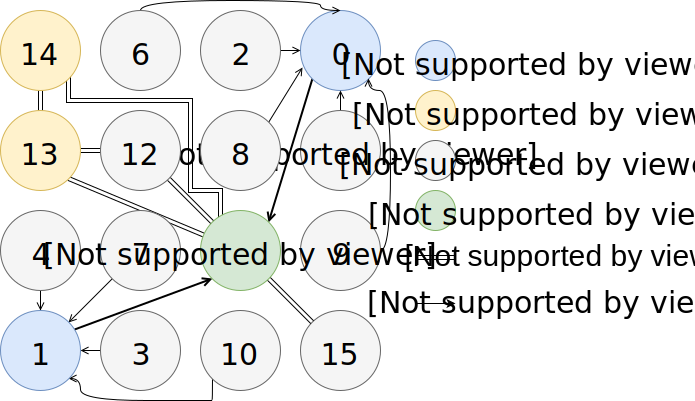
\includegraphics[width=0.7\textwidth]{figures/ContractedSaddle.pdf}
\caption{State of the exemplary 2D dataset after contracting the sub-level set component of 11. 11 was a saddle and now becomes a contracted minimum. In the new setting, the state of saddle candidates can change.}
\label{fig:cons}
\end{figure}

Once a sweep terminates, all vertices in the ascending manifold of the minimum have been visited and the complete boundary of the ascending manifold is considered as potential saddle. Finding the minimum among these potential saddles yields the actual saddle of the minimum. If this saddle is not yet represented by an inner node in the output, such an inner node is created and an edge to the leaf node is established. Otherwise the existing inner node is connected to the leaf with a new edge and a test is performed on the saddle node: 

If all smaller neighbors of the saddle \(s\) have been visited by sweeps of vertices that are descendants of \(s\) in the output, then the connected component that \(s\) belongs to in its sub-level set is completely known and \(s\) is ready to be contracted to a minimum. 

This is simply done by starting a new sweep from \(s\) and considering \(s\) to be connected to every potential saddle of any of its descendants. This is possible because the set of these potential saddles still forms a boundary around the complete level-set component, that \(s\) represents in its sub-level set. This sweep is then treated just like those for a minimum. See Figure \ref{fig:cons}.

Once a sweep terminates without identifying a single potential saddle the algorithm has reached the global maximum and the output is the complete merge tree.
 
\section{Growing the Boundary}
The conclusions in \ref{ssec:num1} state that the ascending manifold of a minimum or saddle \(s\) is always surrounded by saddle candidates, at least one of which will be connecting and the saddle for \(s\). However there can also be saddle candidates inside the ascending manifold. None of these will be a connecting saddle candidate, because the inner candidates' smaller neighbors are also part of the ascending manifold of \(s\) and are therefore reachable by \(s\) through monotone paths. 

\begin{figure}[h!]
\centering
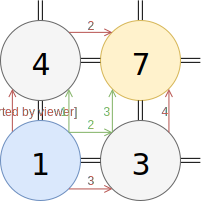
\includegraphics[width=0.5\textwidth]{figures/MultiVisit.pdf}
\caption{The saddle candidate 7 is part of the ascending manifold of 1. Depending on the order of sweep progression, 7 might be temporarily identified as boundary and be checked multiple times.}
\label{fig:mv}
\end{figure}

The existence of these inner saddle candidates complicates the termination criteria for our breadth first search. Instead of just following ascending paths until reaching a saddle candidate, the found saddle candidate needs to be tested, whether any of its smaller neighbors is not part of the ascending manifold. This check however is very simple and computationally not expensive: Just checking whether or not the sweep has already visited all smaller neighbors of the saddle candidate is sufficient. This is because the sweep will visit the complete ascending manifold, thus any reachable smaller neighbors of any saddle candidate. Due to the parallel, unordered nature of the sweep a saddle candidate might be checked before all of its smaller neighbors have been visited, but once the missing smaller neighbors are visited, the saddle candidate will be pushed to the stack of the breadth-first-search again, as it is a larger neighbor of a recently visited vertex. This results in some double work, as saddle candidates might be checked "from" multiple of its smaller neighbors. This double work can be minimized by following ascending paths with preferably small next-to-visit values, e.g. use a priority queue instead of a normal stack for the sweeps. Note that this is a purely performance wise measure and the sweeps can still be parallelized to an arbitrary degree.

A major result of this approach is, that until the sweep is completely terminated, the set of boundary saddle candidates is subject to change. Every time a saddle candidate is reached and checked for the second condition, it is either visited by the sweep or it is added to the set of boundary saddle candidates. It might however be checked again later, when additional smaller neighbors of it has been visited by the sweep. Depending on the order of execution, saddle candidates might be identified as inner candidates only after a second or later check (namely when all of their smaller neighbors have finally been visited). This results in the need for a datastructure holding the set of boundary saddle candidates to allow for insertions and deletions in addition to a final minimum search. 

Lets call this data structure the boundary of a sweep.

\section{Relation to Union-Find}
The algorithm repeatedly relies on the information by which minimum or saddle a certain vertex has been visited, thus to what ascending manifold a vertex belongs. Furthermore the information whether a minimum or saddle is a descendant of another saddle in the output is needed repeatedly. Both question can be efficiently answered by a union find data structure:

This datastructure is typically a reference to a vertex of the input for each vertex of the input (e.g. an array of referenced indices). Whenever a sweep, that started at a minimum or saddle \(s\), visits a vertex \(v\), a trivial union is performed, thus \(v\) points to \(s\) in the data structure. 

Whenever a minimum or saddle \(m\) identifies its saddle \(s\), another union is performed, thus \(m\) points to \(s\). This is a slight difference to a classic union find data structure, as connected components do never unite directly but always point to a common father instead. This difference is also a strong difference between the saddle search breadth-first-search of a minimum and a classic union find scan.

Whenever the information is needed, whether a vertex \(v\) is visited by a minimum or saddle \(s\) or any of its descendants in the output, a find operation is performed. For this the reference chain of \(v\) is followed until either \(s\) or an invalid reference is reached. Since there will be a lot of these queries a path compression is employed, thus any visited node of the reference chain will point to its fathers father after the query.

The operations union and find are therefore utilized in PUMA. The two problems of merge tree construction and union find are closely related, as \cite{pascucci1} is basically a union find variant. However without a global ordering the union find algorithm can only find the total number of connected components in the data, the development of level set components with increasing level are lost, thus the union find algorithm is only a part of PUMA.

Note that in contrast to parallel versions of the union find algorithm, the union find component of PUMA does not require any synchronization. Because a sweep for a saddle \(s\) will only start, once the test for compress-ability returned positive, we know, that any find operations during the resulting sweep, asking for a vertex \(v\) whether it belongs to the component of \(s\), will only ever happen after all descendants of \(s\) in the output are united with \(s\) in the union find datastructure. Thus, if the compress-ability test is sufficiently synchronized, no concurrent union and find operations can impact each others results. Furthermore no concurrent find operations need synchronization, even when considering path compression, as long as reference writes are atomic. Concurrent union operations do not need synchronization either, because of the indirect non-trivial unions via a common saddle.

\section{Augmentation and Ascending Manifolds}
Until now the method for finding the augmentation of the output was neglected. 

To obtain an augmentation, we need to identify for each vertex \(v\) the connected component, that \(v\) belongs to in the sub-level set of the value of \(v\). Each sub-level set component that exists in the input is represented by exactly one edge in the output. Since all edges are between a minimum or saddle \(v\) that started a sweep and the saddle that was found by the sweep, we can label the edges with the index of \(v\). Under this labeling every minimum and saddle in the input will belong to the augmentation of the arc with the same label. 

When sorting the vertices of the input data into sets according to the edge they are augmented to, one receives a complete partitioning of the data set. There is an interesting relation between the partitioning of the data into ascending manifolds and the partitioning into augmentations:

A vertex \(v\) that is part of the ascending manifold of a minimum or saddle \(s\) is either part of the augmentation labeled with \(s\) or of any of the augmentations labeled with vertices that are ancestors of \(s\) in the output. This is apparent, because \(v\) is isolated from all other minima or saddles by the ascending manifold boundary of \(s\). In order for a connection between \(v\) and any minima or saddle \(m\) other than \(s\) to exist in any sub-level set, this sub-level set must contain at least one vertex on the ascending manifold boundaries of \(s\) and \(m\), thus \(s\) and \(m\) must have merged into one sub-level set component in the respective sub-level set. 

In other words in order for a vertex \(v\) to belong to the augmentation of any sub-level set connected component, this component must also include the minimum or saddle in whose ascending manifold \(v\) lies.

Using this knowledge computing the augmentation of the output is easy. Every vertex gets labeled with the minimum or saddle index, when visited by its sweep. When the sweep terminates, all labeled vertices with values greater than the found saddle are labeled with the saddles index instead. This effectively "pushes" all vertices that don't belong in the found arc "up the output tree" to be considered in the next arc. Due to the fact above, vertices will find their respective arc along this path. 

Intuitively the ascending manifolds are "cut" at the value of the found saddle to receive the augmentation.

\section{Merging the Components}
The described process requires us to perform multiple operations, when two or more finished breadth first searches reached a common saddle. 

\begin{figure}[h!]
\centering
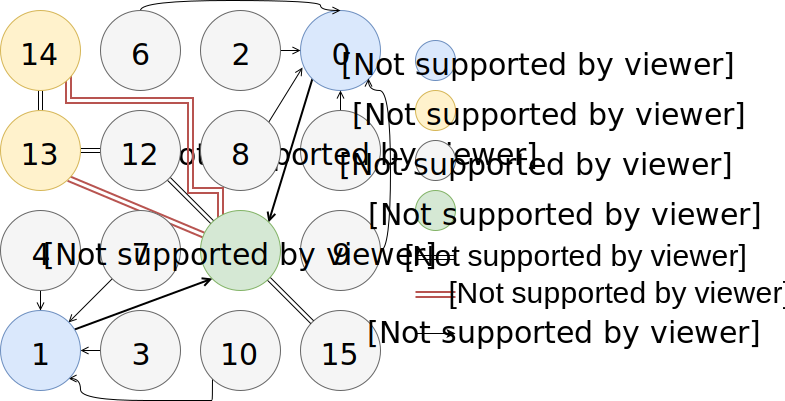
\includegraphics[width=0.7\textwidth]{figures/Unnes.pdf}
\caption{Saddle after contraction of its sub-level set component. Vertices that are only part of at most one child arc boundary need not be initially considered in the new sweep.}
\label{fig:un}
\end{figure}

First, the union find datastructure needs to be updated, so that all (possibly compressed) minima point to their saddle. Second, the set of visited vertices of each sweep needs to be split into two parts. Vertices with a lower value than the saddle will form the augmentation of the finished arc. Vertices with a higher value than the saddle will be added to the set of visited vertices of the upcoming sweep of the saddle. These upper portions of the visited sets of the finished arcs need to be merged into one set before the saddle can start its sweep. Also the sweep of the saddle then needs to update this set with the vertices it visits during the sweep. Thus a datastructure is needed, that allows for fast splitting at a given value, fast merging of multiple instances of the datastructure and concurrent insertion operations. Let's call this datastructure the augmentation of a sweep.

Third the boundaries of the finished breadth first searches need to be merged and added to the initial sweep stack of the saddle. This is the realization of the concept of contracting the connected component of the saddle to one vertex. However this results in a considerable amount of double work, as every vertex on the boundary of every child sweep will be revisited by the saddle sweep. Most of these vertices will still be part of the boundary of the saddle. Only the vertices that, after contraction, would lie within the ascending manifold of the saddle will be actually visited by the saddle sweep. Luckily we can identify vertices that will be part of the boundary of the saddle a priori, without having to check their second condition again:

A vertex that was on the boundary of one of the child sweeps of a saddle, has at least one smaller neighbor that was not part of the ascending manifold of that child. If this smaller neighbor is not part of the contracted saddles ascending manifold, the respective boundary element will persist to be part of the boundary of the saddle. The only two possibilities for the smaller neighbor to be part of the contracted saddles ascending manifold is either by being visited by its sweep later on, or by being already part of the ascending manifold of another child of the saddle. Thus only the vertices that are part of at least two children's boundaries must be checked for the second condition still being met. All vertices that are only part of one child boundary can not have lost their second condition during the contraction and will either remain part of the boundary of the saddle, or be visited later on in the sweep of the saddle.  

Thus instead of adding the complete union of the child boundaries onto the saddles sweep initial stack, only the intersections between the child boundaries are added. All child boundary elements not added that way, are instead added to the initial boundary of the saddles sweep.

\section{Trunk Skipping}
The last important optimization to the algorithm is called trunk skipping:

Due to the nature of the sub-level sets, for every at least two arcs that are identified, only one father arc can start its identification process. While this was a problem for approaches that exposed at most one parallel line of execution per active arc, PUMA should not  more and more sequentialized execution when reaching high nodes in the output. There is however one advantage of this nature, that can be used in both scenarios:

When only one active sweep is left, since all other minima and saddles have identified their saddles, the rest of the computation becomes trivial. There will be a certain amount of "dangling" saddles, that have been identified by some of their children, but not yet by all of them. Since there is only one growing component left, it is clear that this component is the missing child for all of these dangling saddles. Due to Lemma2, we can just order all dangling saddles along their values, connect each with their predecessor in that ordering and finally the smallest one will be the saddle for the last active sweep. 

In a similar fashion the remaining augmentation can be calculated. For that, every vertex that is not yet augmented is sorted into one of the arcs created by the trunk skipping above using their function value. This is correct, because all unvisited vertices must belong to the only growing component that is left, thus the only question remains before and after what joining processes they are added to this component. This sorting process can be parallelized to an arbitrary degree and sped up by using a binary search.


\chapter{PUMA Implementation Details}
The above chapter discussed the design and some optimizations of the novel, unordered approach PUMA. To not disturb the flow of argumentation too much, some implementation details, especially the implementation of the used datastructures was omitted above. The following chapter will clarify the implementation of these data structures and other important details of realization. 

\section{Task-Parallelism}
Up until now, parallelism was treated as an abstract concept. We talked about parallel lines of execution and dependencies only. Therefore an important aspect of the implementation of PUMA is how this parallelism is achieved:

PUMA is a task parallel implementation based on the HPX framework. The task parallel paradigm occurred as a natural fit for the problem. Individual breadth first searches appear as parallely executable parts of the problem -or tasks- and arise and terminate during runtime with mutual dependencies, that are not known a priori. Such a dynamic interdependent set of parallel portions of code can profit strongly from task-parallel concepts such as latency hiding and lightweight context switches as supplied by advanced schedulers like provided by HPX. 

The abstraction of tasks in PUMA is chosen as follows:

Some initial tasks iterate through the dataset in parallel and identify local minima. Every identified local minimum spawns a new task, commissioned to perform the sweep for that minimum. Additional helper tasks could be assigned to a running sweep, when resources become idle, or to control the grain of parallelism. Whenever a sweep terminates, the saddle is checked for contract-ability. If successful this check spawns a new task, commissioned to perform the sweep for that saddle. The dependency graph structure of the tasks is identical to the output tree in this context and of course discovered at runtime.

\section{Global Data Structures}
In order for the different tasks to communicate, several global datastructures are needed. In the following these datastructures, their implementation and usage is explained in detail.

\subsection{Output - Merge Tree}
All tasks must be able to  and modify the current state of the output. Adding leaf nodes for minima, creating or reading existent saddles and creating arcs must be possible through a common, global datastructure. Also the boundary and augmentation datastructures of not yet started saddle sweeps need to be modified by their children, after their sweep finished. All of this must be possible in a concurrent, threadsafe fashion between tasks and with minimal synchronization overhead.

In PUMA this is implemented by aggregating all information relevant for an arc in an "Arc" class. This class holds the (contracted) minimum and saddle of an arc as an index of the respective vertex in the input. It also holds a reference to a boundary datastructure, an augmentation datastructure and an initial stack for the sweep to start on. All of these datastructures are to be filled by finished child arcs by intersecting boundaries and "cutting" augmentations (see above).

To make these arcs globally accessible a complete map from input vertex index to pointers to Arcs is maintained. Since maps are not easily made threadsafe for concurrent use, we trade in some memory for performance: By allocating a complete array of pointers to Arcs with length equal to the number of vertices in the input and initializing the array with null pointers, we can make arcs accessible through the index of their minimum vertex. Creating an Arc for a minimum becomes as trivial as creating an Arc object and creating a pointer in the array at index of the minimum towards that Arc object. Once a saddle is found, it is written to the Arc object and additionally the pointer at the index of the saddle is compared to a null pointer, to see whether the saddle Arc is already created. Now either an Arc object for the saddle is created, or the existing arc saddles augmentation, boundary and search stack are updated. After this the saddle can be checked for contract-ability.

In order to synchronize this global Arc list, a matching list of mutices is created, allowing to lock each index separately. This lock is used to synchronize existence checks of saddle arcs, updating saddle arc datastructures and checking the arc for contract-ability.

\subsection{Union Find Datastructure}
As mentioned above the algorithm relies on a global datastructure maintaining the information what vertex was visited by what sweep. Additionally this same datastructure can be used to store ancestor/descendant relationships of output tree nodes. 

For this purpose another array with length equal to the number of vertices in the input is allocated. Again each position in the array corresponds to the vertex \(v\) with the same index, this time storing an integer with the index of an ancestor vertex \(s\). If \(v\) is not represented by a node in the output tree, \(s\) either started a sweep that visited \(v\) or any descendant of \(s\) in the output tree did, depending on progress of path compression. If \(v\) is represented by a node in the output tree \(s\) is either the saddle found by the sweep of \(v\) or an ancestor of \(v\) in the output tree, depending on progress of path compression. 

This array \(UF\) is initialized with an invalid index for each vertex. Every time a sweep started at a (contracted) minimum \(m\) visits a vertex \(v\), \(UF[v]\) is set to be \(m\). Note that the connecting boundary candidates of the ascending manifolds boundary of \(m\) are not visited in this sense. Thus no two sweep can ever visit the same vertex and these write operations do not require any form of synchronization. 

Every time a sweep started at a (contracted) minimum \(m\) terminates and identifies the saddle \(s\) of \(m\), \(UF[m]\) is set to be \(s\). This operation also requires no form of synchronization, because only the first task finding an empty stack of the sweep of \(m\) will ever write to \(m\).

Find operations are called with two parameters. The first is the index of a vertex \(v\) for which to check whether it is part of the connected component represented by a (contracted) minimum \(s\) with an active sweep. The second parameter is the index of \(s\). The find operation inspects \(UF[v]\) and then \(UF[UF[v]]\) and so forth, until it either finds \(s\) or an invalid index. These read operations require no form of synchronization, not even with the above write operations, because \(v\) either belongs to children of \(s\) or will run into an invalid index at some point. In the first case, all children of \(s\) already terminated their sweep and no write operations to their visited vertices can occur. In the second case read after write and write after read hazards are irrelevant, \(v\) does not belong to \(s\) and will reach an invalid index at some point, whether concurrent write operations delay this result by an additional child-parent relationship being followed or not is of no importance. Lastly path compression does not need any kind of synchronization either. This is because for an entry \(UF[UF[v]]\) to be a valid index, the sweep of \(UF[v]\) needs to be already terminated, thus no concurrent write operations will occur. Concurrent path compression write operations are subject to write after write hazards, however every one of these write operations will write some valid ancestor of \(UF[v]\) and it does not matter in which order this occurs.

Note that the above analysis builds on the assumption, that read/write operations to integers cannot occur amidst concurrent write operations thus reading or creating a bitwise mixture of two valid states. This assumption might only be true on some hardware when using atomic variables.
Additionally the assumption is made, that the writes of terminated child sweeps are visible to the reads of the parent sweep. On some hardware architectures this might require some cache coherency operations to be performed.

\section{Boundary Data Structure}
The use of a datastructure to represent the boundary of a sweep and thus the boundary of an ascending manifold is an essential part of our novel approach. When performing the breadth first search, vertices that are either not saddle candidates or non-connecting saddle candidates are visited, added to the augmentation, updated in the union find datastructure and lastly their non-visited, larger neighbors are pushed to the stack. A non-connecting saddle candidate can however not necessarily be identified the first time it is pulled from the stack, since some of its smaller neighbors might yet be unvisited. Only if a saddle candidate is not connecting, he will be pushed on the stack by all his smaller neighbors and therefore be at some point identified as non-connecting and therefore will be visited. Thus connecting saddles can only be identified by not being visited, when the stack is encountered empty. 

This results in the need to mark or store saddle candidates that were pulled from the stack and not identified as non-connecting and to unmark saddle candidates that were previously marked but then pulled from the stack and identified as non-connecting. Also, finding the minimum among all currently marked saddle candidates, finding the intersection between two sets of marked saddle candidates and lastly finding the union without the intersection between the two are operations needed by the algorithm. This is to identify the saddle and allow this saddle to simulate contraction with minimal double work.

Considering that boundaries might grow very large in practical applications, all operations on the boundary datastructure are highly performance critical. However the main focus should lie on intersection, union and find minimum operations, since these will be performed in a synchronized environment, after child sweeps terminate, while insertion and deletion are part of the parallely executed sweep for each child. 

In accordance with \cite{flatset}, in PUMA the boundary datastructure is implemented as a flat set, more precisely the boost implementation boost:flat\_set is used. In this approach an ordered vector of all inserted elements is maintained. Find operations are implemented through binary search. This allows for constant time minimum identification, due to the ordered nature of the vector. Intersections and unions are done by iterating over the smaller set, searching the current element in the larger set and adding it either to the back of the resulting intersection set or to the larger set. In real data sets the vast majority of join nodes join a very large level set component with a very small one, thus the runtime dependency on the size of the smaller set was very beneficial for the overall runtime. Also a large portion of the join nodes joining two or more major level set components are not relevant for performance, as they are subject to trunk skipping.

Although the theoretical runtime complexity for insertion and deletion operations in the flat\_set is linear, the actual performance impact was rather small. This is most likely due to the inherently (relatively) ordered nature of the algorithm, following ascending paths and constructing the tree bottom up, thus most insertions and deletions in larger boundaries only modify in close proximity to the back of the set. 

In accordance to those considerations boost::flat\_set outperformed std::set, std::unordered\_set and std::bit\_set by an order of magnitude, mainly because of far superior iteration and minimum search times. 

\section{Augmentation Data Structure}
Another important datastructure and aspect of our novel algorithm is keeping track of the arc augmentations. During the sweep, visited vertices are added to the augmentation of that arc. This adds the entire ascending manifold of a minimum or saddle \(m\) to the augmentation of the arc starting in \(m\). The actual set of vertices that belong to the augmentation of that arc is however only a subset of this ascending manifold, and can be obtained from it, by extracting all vertices with a lower value than the found saddle of the arc. The remaining, larger vertices will belong to the augmentation of one of the ancestors of \(m\) in the output tree. Therefore the remaining, larger portion of the ascending manifold are always added to the augmentation datastructure of the saddle of a finished sweep, thus moving upwards the tree, until finding the arc they should be augmented to. The augmentation datastructure therefore needs to support the following operations:

Insertion of vertices, splitting into vertices with smaller and larger values than a splitting threshold respectively and lastly uniting with another instance of the datastructure (to integrate passed on, remaining vertices). Again the focus should lie on operations that can only be done sequentially, once per identified saddle, instead of operations that can be done in parallel for each child individually. This is to try and shift work load "down" the output tree, as work load becomes more and more sequential the higher it occurs in the tree structure.

Gladly there is a datastructure that allows for cutting the augmentation among a saddle value in constant time (after a log(n) find operation): the linked list. Cutting the augmentation is simply performed by cutting a link in the list before the first vertex with a larger value than the saddle. Union operations require us to repeatedly compare the heads of both lists and insert the smaller one at the back of a new list, until one of the united lists is empty and other one can be appended to the new lists tail. Again the inherently (more or less) ordered nature of the algorithm and the typically rather small size of at least one of the two lists strongly benefit this approach, as in most cases one mall list is more or less inserted in one place into the larger list, making the union operation a find operation in the larger list followed by an iteration of the smaller list.

This approach however comes with a huge drawback, as insertions require find operations, which are of linear worst case runtime regarding the size of the lists. This has a tremendous impact on performance, as augmentations may become very large. To tackle this limitation of simple linked lists, a custom implementation of a concurrent skiplist based on \cite{skiplist} was performed. This datastructure allows us to quickly skip large portions of the list, again utilizing the property of insertions usually occurring only near the end of large lists. With skiplists insertion times come again down to a theoretical runtime complexity of log(n) and showed a substantial overall practical runtime improvement. As a skiplist still includes a complete linked list on the lowest layer, union operations worked just the same as before. Cutting the list now theoretically requires log(n) cuts, as this is the height of the list, however performance impacts in cutting times were negligible.

\chapter{PUMA Performance Analysis}
In the sections above we analyzed the consequences of discarding the need for ordered progression in merge tree construction. This led us to a novel algorithm, solving the arising problems of unordered progression, while trying to minimize the performance impact of the additional measures. In the following chapter we will be evaluating these performance impacts and the overall performance of PUMA in comparison to current state of the art implementations of merge tree construction.
\begin{figure}[h]
\centering
\includegraphics[width=0.95\textwidth]{figures/datscale.pdf}
\caption{PUMA runtime scaling with problem size and fitted linear, quadratic and exponential regression for comparison.}
\label{fig:datscale}
\end{figure}

\section{Scalability with Problem Size and Resources}
While it is not in the scope of this thesis to formally prove the theoretical runtime complexity of the presented solution, there is a particularly interesting consequence of unordered progression in PUMA, that impacts runtime complexity:

In PUMA the ascending manifold boundary of merge tree nodes is used to identify saddles and simulate saddle contraction. While an effort was made to minimize performance impact of these operations, the theoretical runtime complexity of some of these operations can only be given an upper bound of quadratic runtime in the size of the boundary. When considering the typical approach of input data being represented by a 3D regular grid, ascending manifold boundaries represent 2D surfaces in this grid. Since the problem size \(n\) (number of vertices in the input data) grows cubically with the resolution of the regular grid in each dimension and the surface sizes \(m\) within the grid will grow quadratically with the resolution \(n\) and \(m\) will have the following asymptotic growth relationship: \(O(m) =O(n^{2/3})\). With the quadratic runtime dependency of the boundary sizes of some operations in PUMA the runtime of PUMA cannot be bounded by an upper bound smaller than \(O(n^{4/3})\).

Figure \ref{fig:datscale} shows runtimes of PUMA on a dataset that is resampled to different resolutions in order to analyze the practical scalability of PUMA with problem size. In this evaluation 8 threads on the 4 cores of an Intel(R) Core(TM) i7-6700K CPU were run. Note that the x-axis of the plot positions the different problem sizes equidistantly and not to scale of their size, this is to increase visual clarity of the plot. To give a frame of reference for the growth, a linear, quadratic and e-exponential regression are plotted in comparison. Both linear and quadratic regression achieve correlation factors above 0.99 with the factor for the quadratic term in the quadratic regression being as low as \(4*10^{-16}\). This implies a real world scalability with close to linear behaviour.

\begin{figure}[h]
\centering
\includegraphics[width=0.95\textwidth]{figures/resscale.pdf}
\caption{PUMA runtime scaling with number of utilized OS-Threads}
\label{fig:resscale}
\end{figure}

On the same hardware, PUMA was run with varying numbers of utilized operating system threads to demonstrate small scale parallel abilities. Note that the far smaller speedup increase when going from 4 to 8 threads is most likely due to the additional 4 operating system threads being only realized through hyper-threading. 

The super-linear speedup achieved could be explained by effects of trunk skipping: Consider a very large leaf arc that has a size far greater than the second largest leaf arc. A purely sequential execution will work through arcs in a strict ordering, for example given by index of local minimum vertices. Since trunk skipping will only skip the work for the last active arc, the effect of trunk skipping is dependent on how large the arc for the last encountered local minimum is. In a parallel execution, large arcs will be active much longer than small arcs, thus -assuming random ordering of arcs- the probability for an arc to be the last active arc scales with its size. Thus in parallel execution the chance for trunk skipping to skip a rather large portion of work is higher than in sequential execution. 

This can easily be understood, when considering an extreme example. Consider a dataset resulting in only 3 very small arcs and one very large arc (that finally collects the other 3 arcs at inner nodes along the trunk). When run sequentially the chance for the large arc to be trunk-skipped is only one fourth, when run with 4 threads, running one task each, it is guaranteed that the large arc is skipped once the three smaller arcs terminate their construction.

\section{Runtime Comparisons}
Figure \ref{fig:runtime} shows relative runtime of three different merge tree construction algorithms:

While TTK Contour Forests is a solution representing traditional divide-and-conquer approaches with global sorting per segment, TTK FTM is the implementation of the algorithm in \cite{FTM}. Additionally the reeb graph computation provided in the VTK framework was benchmarked, however only runtimes for the subsampled dataset "ctBones small" could be measured in reasonable time and would correspond to over two thousand times the runtime of TTK Contour Forests. All datasets are 3D regular grids, except for the dragon dataset, which is a mesh. This is the reason why no runtime for TTK FTM on the dragon dataset could be measured, as the TTK FTM does not support this datatype. 

\begin{figure}[h]
\centering
\includegraphics[width=0.85\textwidth]{figures/runtime.pdf}
\caption{PUMA runtime in comparison with TTK Contour Forests and TTK FTM.}
\label{fig:runtime}
\end{figure}

As can be seen the task-parallel, decentralized approach of FTM outperforms  traditional approaches, as also observed in \cite{FTM}. PUMA being very similar to FTM is able to reproduce this performance gain on some datasets, however a clear penalty for the maintenance of additional datastructures can be observed. Additionally as PUMA's runtime is very dependent on boundary sizes, especially when two components with very large boundaries merge, a strong variation in relative performance depending on the data can be observed to be present in PUMA. 


\section{Conclusion}
As discussed above, discarding the need for ordered progression during merge tree construction introduces some additional complications to the algorithmic structure. Keeping track of boundaries and allowing prematurely augmented vertices to be updated whenever a saddle is found does come with additional computational effort. In exchange for that, no ordering needs to be maintained and a single arc construction could be parallelized, allowing for potentially better scaling with available resources. However in realistic datasets that are prone to noise, the huge majority of arcs is very small, as in having a small augmentation and ascending manifold per minimum or saddle. Arcs large enough to justify the parallelization overheads of PUMA are typically subject to trunkskipping anyway, leaving little room for PUMAs advantages to contribute to better runtimes. 

However, increased theoretical scaling with resources is not the only benefit, that arises from discarding the need for ordering in merge tree construction. In some scenarios where an ordered progression is just not feasible, the ground concept of PUMA can be highly beneficial to implement a parallel, bottom up merge tree construction. 

One of the most important of these scenarios is distributed merge tree construction on clusters and for segmented data in general. Consider a distributed environment holding different segments of the data per computation node, as for example with in-situ or out-of-core scenarios. In the locally ordered paradigm of \cite{FTM}, each arc extends the ascending paths in order of their values. If ascending paths of a single arc span multiple segments of data, the algorithm can only proceed in one data segment at a time. This results in heavy sequential dependencies on round-trip times (in-situ) or data segment loading times (out-of-core) to a degree, where the discussed decentralized bottom-up construction methods become unfeasible. This conclusion fits well with the observation, that all distributed merge tree construction algorithms known to the authors at the time of writing employ a divide and conquer, data-parallel approach, even though task-parallel sweep-based approaches like in \cite{FTM} show superior potential in both sequential and parallel scenarios. 

The focus of this thesis shall however be another scenario, where ordered progression is not feasible: The SIMT environment of GPGPUs. With the large amount of computational nodes, the limitation of one parallel line of execution per arc of locally ordered approaches becomes all the more impactful. Additionally with the constrained memory versatility on these platforms, executing an ordered search through a graph becomes unfeasible. In the following chapters a hardware accelerated variant of PUMA (GPUMA) is discovered to serve as a proof of concept, showcasing the ability of an unordered merge tree construction approach to utilize hardware that would suffer severely from dependencies on ordered progression. 

\chapter{GPUMA}
In the following section the adaption of the PUMA algorithm explained above to the platform of an SMP environment, more precisely the SIMT model of NVIDIA GPGPUs is discussed. Please note, that GPUMA does not aim to be an optimal solution for merge tree construction on SMP architectures, but rather an adaption of PUMA to such an architecture for demonstration of the versatility of the new approach. A very similar solution to GPUMA, that is inherently stronger tailored towards SMP architectures is discussed in \cite{Carr}. There, ascending manifolds are identified by following paths towards extrema and not starting at extrema like done here. This leads to ascending manifold boundaries to be associated with either of their reachable extrema and creates the need for a more global perspective when identifying saddles. To avoid misunderstandings \cite{Carr} uses the term saddle candidate only for what is called connecting saddle candidate here. Non-connecting saddle candidates are of no concern in the approach in \cite{Carr}.

\section{Round Based vs. Megakernel}
While the parallelism of PUMA utilizes a purely task-based implementation, simply migrating the cpu code into a single megakernel would come with a lot of limitations. It would be possible to populate a central work stack with (contracted) minima and let one large kernel pull from this stack, starting the complete task of arc construction for each work stack element. However different portions of these tasks interact with other portions in a very dynamic way, creating for example the need for a union find datastructure. To minimize in-warp divergence and the need for dynamic datastructures, the tasks are split up into portions with simple mutual interaction and interaction with different task portions is avoided, by synchronizing task progression to a round based approach. This approach is in accordance with observations made in \cite{megakernel}.

\section{Structure}
The general structure of GPUMA is very similar to PUMA. 

\subsection{Minimum Search}
At first a search for global minima is performed. Instead of instantly submitting a construction task for each found minimum, all minima are collected in a stack. Only after the complete dataset was scanned for minima the next step is performed, thus a simple atomic counter is enough to synchronize the global work stack. As with all of the following kernels, register use is fairly limited and due to the close relation to a task based solution the number of threads to use is completely arbitrary. In order to allow for maximal latency hiding and occupancy the maximum number of threads available per SM is spawned in as few blocks as possible.

\subsection{Arc Growth}
A second kernel then pulls minima from the stack and grows their ascending manifolds by performing a sweep just like described in PUMA. Again a simple atomic counter is enough to synchronize the sweep stack as no ordering is needed. To avoid dynamic memory allocations in this phase, the stack size of the sweep is limited. When a sweep encounters a full stack, it is automatically transferred to the next round (see \ref{ssec:num2}). Thanks to the round based approach neither a datastructure for the boundary nor the augmentation needs to be maintained. Only the union find datastructure needs to be updated and thanks to the compressed nature of the union find datastructure in GPUMA both union and find operations will only ever resolve one pointer (see below). As this step is basically a conditioned graph traversal, memory access efficiency and divergence are expected to be rather suboptimal. 

\subsection{Making Boundaries Implicit}
In a third step the whole dataset is scanned again to identify saddles. This is easily possible because after the ascending manifolds are constructed, every vertex that has at least two neighbors from different manifolds is a connecting saddle. Participating in atomic minimum operations for the respective manifolds minima will yield the saddle for each minimum. In a second scan over these saddle candidates, comparing each candidate to the result of the mutual minimum operation, the actual saddle is added to the next work stack and the union find datastructure is updated. This step allows for saddle identification without keeping track of the boundary for each manifold explicitly, thus removing the need for complex, dynamic datastructures.

\subsection{Extracting Boundary Intersections}
For contraction simulation again a scan over the saddle candidates is run, but every vertex on the intersection of two children's boundaries of the same saddle is added to a list of start locations for that saddles' sweep. Because this requires some dynamic memory allocations, this phase is also used to transfer full sweep stacks into similar start location lists for every manifold that is transferred to the next round (see \ref{ssec:num2}). This step actually requires three scans to be performed. The first increments a counter for every element that wants to be added to a start location list of a saddle. The second one iterates over the saddles and dynamically allocates lists with the respective size. The third one iterates again over the saddle candidates and adds them to their respective position in the start location lists.

\subsection{Making Union-Find Compressed}
Iterating again over the complete dataset the union find datastructure is completely path compressed, by letting every entry with a valid fathers father point to this grandfather directly. This is sufficient as this step is repeated every round and only one step in the hierarchy of the union find datastructure can be added per round. This opportunity is also used to compare each vertex that is not yet augmented with the value of this grandfather. If the observed vertex has a value smaller than the grandfather, it belongs to its augmentation and the global augmentation datastructure is updated. This eliminates the need to keep track of augmentations per arc and avoids the use of complex, dynamic datastructures like the skiplist of PUMA.

\section{Sustaining Large Arcs Through Rounds}\label{ssec:num2}
After the above steps, a new round is started by now growing the arcs of the identified saddles. This static round structure however comes with huge limitations. First, if we forced an arc growth to be finished before continuing with the next phase, a statically sized stack for the sweep would not suffice and the need for more dynamic datastructures would arise. Second, round length would be determined by the longest current arc growth, creating the possibility for huge load imbalance. Also in the case of the largest arc of a certain height in the tree being far larger than the remaining arcs with that height, the effectiveness of trunk skipping would be drastically reduced, as skipable arcs would be required to finish before continuing with the next round.

In order to overcome these limitations arc growths are allowed to be interrupted to allow for progression to the next phase. This way small to medium sized arcs will identify their saddle within one round, until not enough arcs remain to keep occupancy high enough. Remaining arc growths (or these with a full stack) are then ignored when identifying boundaries and saddles and instead their stack is transferred to a dynamically allocated list. As tasks can now sustain through rounds of bundled global computations load imbalance is cancelled out. 

\section{Memory Layout}
As most phases iterate over the complete dataset and work on values of neighbors for each vertex, some inherent local coherence in memory accesses is present. To somewhat counteract the rather incoherent access patterns of graph traversal and neighbor comparisons present in most kernels, vertex values were represented with a cudaArray3D. This datastructure specializes in semi-random access patterns on three dimensional data with some local coherence. Memory access efficiency perceived a strong benefit from this and overall runtime was reduced by as much as fifteen percent on average. 

\section{Passing Back to CPU}
As with increasing height in the tree the number of active arc growths becomes smaller, the GPU becomes less and less optimal for the computation. One big reason for this, is that boundary intersection sizes grow, making the penalty of dynamic allocations more and more severe. Another big reason is, that even though a single arc growth could be parallelized, a synchronization between blocks on the GPU is not possible and not all tasks can work on just a few arcs on the GPU if we want to utilize the maximum number of threads. Thus it seems reasonable to transfer the problem in this late stage back to the CPU to utilize its higher single core performance in these inherently sequential stages. Since PUMA requires complete information about boundary and augmentation status, we chose a quickly assembled implementation of the ideas in \cite{FTM} to finish this final stage. 

\begin{figure}[h]
\centering
\includegraphics[width=0.95\textwidth]{figures/gruntime.pdf}
\caption{GPUMA runtime in comparison with PUMA, TTK Contour Forests and TTK FTM. Benchmarks were performed on an NVIDIA GeForce GTX 1080.}
\label{fig:runtime}
\end{figure}


\section{GPUMA Performance Comparison}
Although there is a graph traversal at the heart of PUMA, making semi-random memory accesses the main performance bottleneck and additionally the need for dynamic memory allocations could not be eliminated entirely, the GPU realization of PUMA does perform feasibly well. While memory access efficiency and divergence were suboptimal in some kernels, dropping as low as 15\% memory efficiency and 30\% divergence efficiency, overall occupancy was far above 90\% for all kernels and after three rounds of GPUMA typically 90\% of arcs in the dataset were computed. Depending on dataset the speedup from PUMA to GPUMA achieved up to x20 surpassing runtimes of the locally ordered CPU solution TTK FTM. Please note, that the dragon dataset's overall runtime was in the milliseconds for each algorithm and GPUMA suffers from some initial overhead because of host device communication, which is also in the milliseconds, making GPUMA perform relatively badly on this small dataset.


\chapter{Conclusion and Future Work}
As both contemporary datasets and hardware grow in size and complexity, algorithms for automatic data analysis and visualization and methods for their scalable parallelization become more and more important. Many of these algorithms depend on topological abstractions of the data, as for example the contour tree. 

In the last two years contour tree construction has seen some improved and scalable implementations tailored for various hardware architectures, all of which were based on novel but similar approaches, constructing merge trees in a decentralized way focusing on monotone paths between critical points \cite{origin}. 

In this paper we recaptured the theoretical background that is a common ground behind these recent approaches, by establishing three observations about saddles. First, connected nodes in a merge tree are always connected through a monotone path in the dataset. Second, a merge node always has neighbors in the dataset that are not reachable by a monotone path from all of the components merging at them. Third, the smallest/largest vertex fulfilling these conditions with respect to a component is its join/split node. 

Extending upon these saddle conditions we made observations about the relation of the merge tree construction to the morse theory concept of ascending manifolds. These relations allowed us to introduce a novel task-parallel contour tree construction algorithm that does not depend on any global or local ordering of vertices and minimizes dependency on sharing global information in a shared memory, appearing very well suited for distributed, in-situ, out-of-core or SMP environments. While the new approach comes with some additional complexity, efforts were undertaken to minimize performance impact of these new complications. Performance evaluation showed, that the resulting implementation "PUMA" constructed merge trees in time comparable to the most recent and performant known implementations. 

To prove the adaptability of this novel implementation to different hardware settings, it was adapted to run on SMP architectures and implemented with CUDA. Performance evaluation on an NVIDIA graphics card showed runtime speedups of up to 20x, demonstrating the feasibility of the approach.

Following these observations, efforts and this prove of concept, the presented novel algorithm appears as a promising candidate to be adapted to HPC environments, utilizing task-parallel benefits such as latency hiding, while minimizing dependencies between local chunks of data by eliminating the need for ordering during progression. Future work should therefore include the adaption of PUMA to distributed, in-situ or out-of-core settings and environments, evaluating its performance, scalability and potential to integrate load balancing techniques. 

% --------------------------
% Back matter
% --------------------------
{%
\setstretch{1.1}
\renewcommand{\bibfont}{\normalfont\small}
\setlength{\biblabelsep}{0pt}
\setlength{\bibitemsep}{0.5\baselineskip plus 0.5\baselineskip}
\printbibliography
}
\cleardoublepage
\clearpage
\newpage
\mbox{}

% **************************************************
% End of Document CONTENT
% **************************************************
\end{document}

